%\documentclass[compress]{beamer}
\usepackage{pgfpages}
\usepackage{etex}
\usepackage[utf8]{inputenc}

\mode<article>
{
  \usepackage{fullpage}
  \usepackage{pgf}
  \usepackage{hyperref}
}

\mode<presentation>
{
  \usetheme{metuceng}
  \setbeamercovered{transparent}
}


\title{CEng 242, Programming Language Concepts}
\author{Onur Tolga Şehitoğlu}
\institute[METU]{Computer Engineering}
\subtitle{Introduction}
\date{}

\titlegraphic{\insertmetutitle\insertlicense}

\begin{document}
\frame[plain]{\maketitle}
\section{Introduction}
\begin{frame}
\frametitle{Introduction}
\begin{itemize}
 \item Church-Turing hypothesis say all programming languages and computational devices have the same power regarding computability.
\item If you can define a computation in one of the universal programming languages, you can define the same computation in any other universal programming language. 
\item Why do we have so many programming languages?
\item Is it desirable to know as much distinct P.L. as possible?
\end{itemize}
\end{frame}

\section{Course Objectives}
\begin{frame}
 \frametitle{Course Objectives}
\begin{itemize}
 \item {\em Not\/} to teach specific programming languages. \textsf{Haskell}, \textsf{C++} and \textsf{Prolog} languages are tools of this course.
\item  Studying the common concepts of programming languages.
\item Studying the different paradigms and approaches.
\item What is the measure of \textbf{quality} in a programming language?
\item Construct a basis for other topics like compiler design, software engineering, object oriented design, human computer interaction...
\end{itemize}
\end{frame}

\begin{frame}
 \frametitle{Related Areas}
\begin{itemize}
 \item Human computer interaction
\item Operating systems
\item Computer Architecture
\item Databases and information retrieval
\item Software engineering
\end{itemize}
\end{frame}

\section{Programming Languages vs Natural Languages}
\begin{frame}
 \frametitle{Programming Languages vs Natural Languages}
\begin{itemize}
 \item Formal vs Informal
\item Strict rules of well-formedness vs Error tolerant
\item Restricted vs Unrestricted domain
\end{itemize}
\end{frame}

\section{Features of a Programming Language}
\begin{frame}
 \frametitle{What makes a language programming language?}
Is any formally defined language a programming language?
(HTML?)
\begin{itemize}[<+->]
 \item \textbf{Universal:} All computation problems should be
expressable.\\ \pause
	condition+(loop and/or recursion)
\item \textbf{Natural:} All features required for the application domain.\\
	Fortran: numerical computation, COBOL: file processing, LISP tree and list operations.
\item \textbf{Implementable:} It is possible to write a compiler or interpreter working
on a computer.\\
Mathematics, natural language?
\item \textbf{Efficient:} Works with acceptable amount of CPU and memory.\\
\end{itemize}
\only<5->{\scriptsize ``Hello world'' in different languages:\\
\url{https://helloworldcollection.github.io/}}
\end{frame}

\section{Paradigms}
\begin{frame}
\frametitle{Paradigms}
\textbf{Paradigm:} Theoretical or model frame. A model forming a basis for all
similar approaches.
\begin{itemize}
 \item \textbf{Imperative} Fortran, Cobol, Algol, Pascal, C, C++, Java, Basic.
\item \textbf{Functional} Lisp, Scheme, ML, Haskell, Miranda
\item \textbf{Object Oriented} Smalltalk, C++, Object Pascal, Eifell, Java, Csharp.
\item \textbf{Concurrent} Ada, Occam, Par-C, Pict, Oz
\item \textbf{Logic} Prolog, Icon
\item \textbf{Constraint Programming} CLP, CHR
\item \textbf{Mixed} Parallel Prolog, Oz (A functional, logic, object oriented, concurrent language: {\tt http://www.mozart-oz.org})
\end{itemize}

\end{frame}

\section{Syntax and Semantics}
\begin{frame}
 \frametitle{Syntax and Semantics}
\begin{itemize}
 \item \textbf{Syntax} Form. How language is structured, how it is expressed.
\item Syntax is represented by Context Free Grammars expressed in BNF (Bacus Naur Form) notation (See CEng 280, Formal Languages and Abstract Machines)
\pause
\item \textbf{Semantics} What does a program mean? How it works.
\end{itemize}
\end{frame}

\section{Language Processors}
\begin{frame}
\frametitle{Language Processors}
\begin{itemize}
\item Compilers (gcc, javac, f77)
\item Interpreters (scheme, hugs, sml, bash)
\item Beautifiers, pretty printers (a2ps, ident)
\item Syntax directed editors (vim, anjuta, eclipse, visual studio)
\item Validators (vgrind, lint)
\item Verifiers 
\end{itemize}
\end{frame}

\section{History}
\begin{frame}
\begin{tabular}{lp{20em}}
%\includegraphics[height=\textheight]{histtalen2}
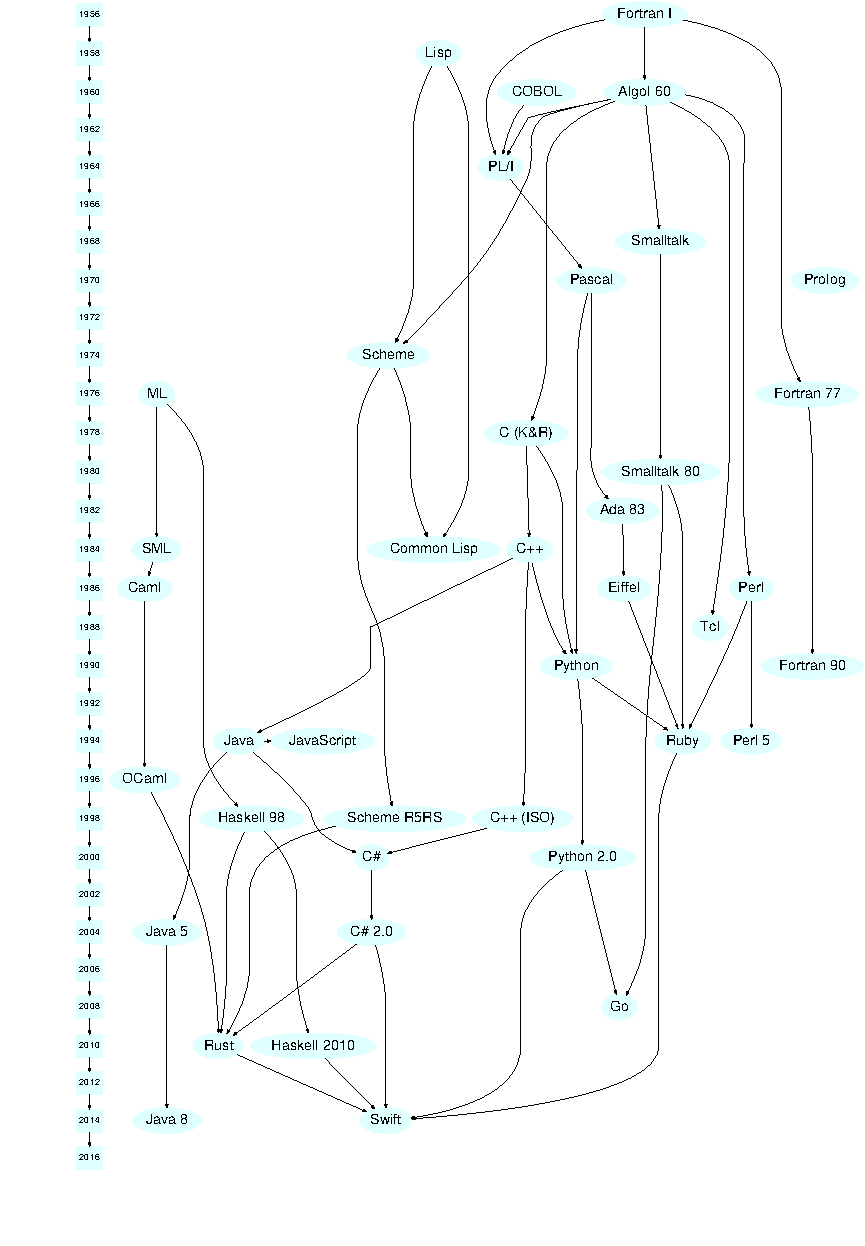
\includegraphics[height=\textheight]{diagram-light} &
{\fontsize{4}{5} \selectfont \shortstack[l]{Taken from: \\
	\url{http://rigaux.org/language-study/}\\[2em]
	O'reiley poster:\\
	http://archive.oreilly.com/pub/a/\\
	oreilly/news/languageposter\_0504.html\\
	\href{http://cdn.oreillystatic.com/news/graphics/prog_lang_poster.pdf}{download link}\\[10em]
	}}
\end{tabular}
\end{frame}
\end{document}
